%%%%%%%%%%%%%%%%%%%%%%%%%%%%%%%%%%%%%%%%%
% Beamer Presentation
% LaTeX Template
% Version 1.0 (10/11/12)
%
% This template has been downloaded from:
% http://www.LaTeXTemplates.com
%
% License:
% CC BY-NC-SA 3.0 (http://creativecommons.org/licenses/by-nc-sa/3.0/)
%
%%%%%%%%%%%%%%%%%%%%%%%%%%%%%%%%%%%%%%%%%

%----------------------------------------------------------------------------------------
%	PACKAGES AND THEMES
%----------------------------------------------------------------------------------------

\documentclass{beamer}

\mode<presentation> {

% The Beamer class comes with a number of default slide themes
% which change the colors and layouts of slides. Below this is a list
% of all the themes, uncomment each in turn to see what they look like.

%\usetheme{default}
%\usetheme{AnnArbor}
%\usetheme{Antibes}
%\usetheme{Bergen}
%\usetheme{Berkeley}
%\usetheme{Berlin}
%\usetheme{Boadilla}
%\usetheme{CambridgeUS}
%\usetheme{Copenhagen}
%\usetheme{Darmstadt}
%\usetheme{Dresden}
%\usetheme{Frankfurt}
%\usetheme{Goettingen}
%\usetheme{Hannover}
%\usetheme{Ilmenau}
%\usetheme{JuanLesPins}
%\usetheme{Luebeck}
\usetheme{Madrid}
%\usetheme{Malmoe}
%\usetheme{Marburg}
%\usetheme{Montpellier}
%\usetheme{PaloAlto}
%\usetheme{Pittsburgh}
%\usetheme{Rochester}
%\usetheme{Singapore}
%\usetheme{Szeged}
%\usetheme{Warsaw}

% As well as themes, the Beamer class has a number of color themes
% for any slide theme. Uncomment each of these in turn to see how it
% changes the colors of your current slide theme.

%\usecolortheme{albatross}
%\usecolortheme{beaver}
%\usecolortheme{beetle}
%\usecolortheme{crane}
%\usecolortheme{dolphin}
%\usecolortheme{dove}
%\usecolortheme{fly}
%\usecolortheme{lily}
%\usecolortheme{orchid}
%\usecolortheme{rose}
%\usecolortheme{seagull}
%\usecolortheme{seahorse}
%\usecolortheme{whale}
%\usecolortheme{wolverine}

%\setbeamertemplate{footline} % To remove the footer line in all slides uncomment this line
%\setbeamertemplate{footline}[page number] % To replace the footer line in all slides with a simple slide count uncomment this line

%\setbeamertemplate{navigation symbols}{} % To remove the navigation symbols from the bottom of all slides uncomment this line
}

\usepackage{graphicx} % Allows including images
\usepackage{wrapfig} 
\usepackage{booktabs} % Allows the use of \toprule, \midrule and \bottomrule in tables
\usepackage{algorithm}
\usepackage{amsmath}
\usepackage{algpseudocode}
\usepackage{mathtools}
\usepackage{bibentry}


%\usepackage[usenames, dvipsnames]{color}


\newcommand\Fontvi{\fontsize{8}{7.2}\selectfont}
\newcommand\fontbig{\fontsize{15}{7.2}\selectfont}

%----------------------------------------------------------------------------------------
%	TITLE PAGE
%----------------------------------------------------------------------------------------

\title[]{Continuous-time Perspectives on Accelerated First-Order Methods} % The short title appears at the bottom of every slide, the full title is only on the title page
\author[Chan, Dean, Pacchiano, Tripuraneni]{Jeffrey Chan, Sarah Dean, Aldo Pacchiano, Nilesh Tripuraneni} % Your name
\institute[UCB] % Your institution as it will appear on the bottom of every slide, may be shorthand to save space
{Department of EECS,
University of California, Berkeley }
\date{\today} % Date, can be changed to a custom date

\begin{document}

\begin{frame}
\titlepage % Print the title page as the first slide
\end{frame}


%\begin{frame}
%\frametitle{Overview} % Table of contents slide, comment this block out to remove it
%\tableofcontents % Throughout your presentation, if you choose to use \section{} and \subsection{} commands, these will automatically be printed on this slide as an overview of your presentation
%\end{frame}

%----------------------------------------------------------------------------------------
%	PRESENTATION SLIDES
%----------------------------------------------------------------------------------------

%------------------------------------------------
% Sections can be created in order to organize your presentation into discrete blocks, all sections and subsections are automatically printed in the table of contents as an overview of the talk
%------------------------------------------------

%------------------------------------------------
\section{Introduction}

\begin{frame}
\frametitle{ Gradient Descent }
\begin{block}{Gradient Descent}
First-order method to minimize $f:\mathbb{R}^n \rightarrow \mathbb{R}$.
\begin{align*}
    x_{k+1} = x_k - s \nabla f(x_k)
\end{align*}
\end{block}

\begin{center}
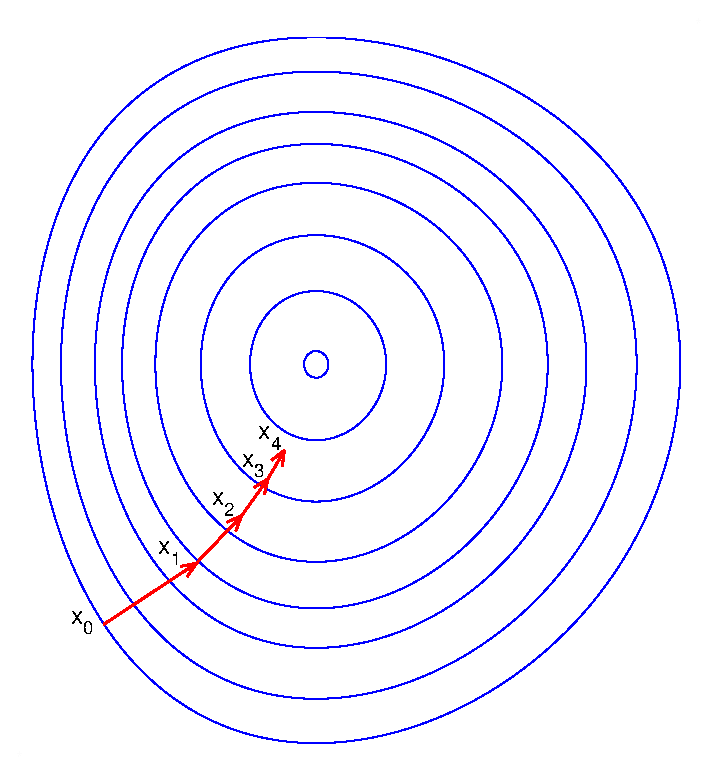
\includegraphics[width=2in]{SourceFiles/plots/Gradient_descent.eps}
\end{center}
\end{frame}

\begin{frame}
\frametitle{ Smoothness and Strong Convexity }

\begin{block}{$\beta$-Smoothness}
$f$ is $\beta$-smooth if:
\begin{align*}
f(y) \leq f(x) + \nabla f(x)^\top(y-x)+ \frac{\beta}{2} ||x - y||_2^2
\end{align*}
\end{block}



\begin{block}{$\alpha$-Strong Convexity}
$f$ is $\alpha$-strongly convex if:
\begin{align*}
f(y) \geq f(x) + \nabla f(x)^\top(y-x) + \frac{\alpha}{2} ||x - y||_2^2
\end{align*}
\end{block}

\begin{block}{Condition number}
Condition Number $\kappa = \frac{\beta}{\alpha}$ for a $\beta$-Smooth and $\alpha-$Strongly Convex function.
\end{block}
\end{frame}

\begin{frame}
\frametitle{Gradient Descent Convergence Rates}

\fontbig

\begin{block}{Convergence Rate}
$f(x_k) - f(x^*) \lesssim \mathcal{O}(\text{ rate })$ 
\end{block}

\fontbig

\begin{center}
 \begin{tabular}{||c c ||} 
 \hline
 Function Class  & GD convergence rate \\ [0.5ex] 
 \hline\hline
 $\beta$-Smooth  & $\frac{1 }{k}$  \\ [1ex]
 \hline
 $\beta$-Smooth, $\alpha-$Strongly Convex   & $\exp\left(-\frac{k}{\kappa}\right)$  \\[1ex]
 \hline
\end{tabular}

\end{center}

\fontbig

\begin{block}{Can we do better?}
\onslide<2->Yes! -- ``Accelerate"
\end{block}

\end{frame}



\begin{frame}

\frametitle{Nesterov's ``Accelerated" Gradient}


\begin{block}{Nesterov's Accelerated Gradient (I)}
For $f$ $\beta$-smooth functions:
\begin{align*}
    x_k =& y_k - s \nabla f(y_{k-1}) \\
    y_k =& x_k + \frac{k-1}{k+2}(x_k - x_{k-1})
\end{align*}
\end{block}

\begin{block}{Nesterov's Accelerated Gradient (II)}
For $f$ is $\beta$-smooth and $\alpha$-strongly convex:
\begin{align*}
x_k =& y_{k-1} - \frac{1}{\beta} \nabla f(y_{k-1})\\
y_k =& x_k + \frac{\sqrt{\kappa} - 1}{\sqrt{\kappa}+1} (x_k - x_{k-1})
\end{align*}

\end{block}

\Fontvi
*We can do this also for noneuclidean geometries via Mirror descent \cite{DBLP:journals/ftml/Bubeck15}.  

\end{frame}



\begin{frame}
\frametitle{``Accelerated" Gradient Descent Convergence Rates}
\fontbig
\begin{center}


 \begin{tabular}{||c c c c ||} 
 \hline
 Function Class   & GD  &  Nesterov  \onslide<2-> {& Lower bound }\\ [0.5ex] 
 \hline\hline
 $\beta$-S & $\frac{1}{k}$ & \textcolor{blue}{$\frac{1}{k^2}$} & \onslide<2->{ \textcolor{blue}{$\frac{1}{k^2}$} } \\ [1ex]
 \hline
 $\beta$-S, $\alpha-$SC  &  $\exp\left(-\frac{k}{\kappa}\right)$ & \textcolor{red}{$\exp\left(-\frac{k}{\sqrt{\kappa}}  \right)$} & \onslide<2-> {\textcolor{red}{ $\exp\left(-\frac{k}{\sqrt{\kappa}}  \right)$} }\\ [1ex]
 \hline
\end{tabular}



\end{center}



\begin{block}{Can we do better?}
\onslide<2-> {Not with a first order method \cite{DBLP:journals/ftml/Bubeck15}, \cite{nesterov2004introductory}.}
\end{block}

%*People are interested in the continuous limit of these methods. This kind of approach was started by Candes in their 2015 paper. They study the top row of the table. We provide results regarding the bottom part of the table. 


\end{frame}

\section{Continuous-Time Limits}

\begin{frame}
\frametitle{An ODE for Gradient Descent \cite{su2014differential}}
\begin{block}{Limit of Gradient Descent}
\begin{center}
$x_k \approx X(\overbrace{k s}^{t})$ for the curve $X(t)$: \\
\begin{align*}
\begin{rcases*}
    x_k &= x_{k-1} - s \nabla f(x_{k-1}) \\
\end{rcases*} \overset{s \to 0}{\longrightarrow} \dot{X} = - \underbrace{\nabla f(X)}_{``force"}
\end{align*}
\end{center}
\end{block}

\begin{block}{Lyapunov Functional (Weakly Convex) -- \cite{su2014differential}}
$\textcolor{red}{t} (f(X(t)) - f(x^*)) + \frac{1}{2}||X(t)-x^*||^2 \implies f(X(t))-f(x^*) \lesssim \mathcal{O}(\frac{1}{\textcolor{red}{t}})$
\end{block}

\begin{block}{Lyapunov Functional (Strongly Convex) -- [Us!]}
$e^{- \textcolor{red}{\alpha} t} (f(X(t)) - f(x^*)) + \frac{1}{2}||X(t)-x^*||^2) \implies f(X(t))-f(x^*) \lesssim \mathcal{O}(e^{-\textcolor{red}{\alpha} t})$
\end{block}


\end{frame}


\begin{frame}
\frametitle{An ODE for Nesterov Acceleration (I) \cite{su2014differential}}
\begin{block}{Limit of ``Accelerated" Gradient Descent (for Weakly Convex $f$)}
\begin{center}
$x_k \approx X(\overbrace{k\sqrt{s}}^{t})$ for the curve $X(t)$: \\
\begin{align*}
\begin{rcases*}
    x_k &= y_{k-1} - s \nabla f(y_{k-1})\\
    y_k &= x_k + \frac{k-1}{k+2} (x_k - x_{k-1}) 
\end{rcases*} \overset{s \to 0}{\longrightarrow} \underbrace{\ddot{X}}_{``mass"} + \underbrace{\frac{3}{t} \dot{X}}_{``damping"} + \underbrace{\nabla f(X)}_{``force"} = 0
\end{align*}
\end{center}
\begin{itemize}
    \item ``Small" $t$: large ``damping" $\implies$ fast decay to equilibrium
    \item ``Large" $t$: small ``damping" $\implies$ fast oscillations toward optima
\end{itemize}
\end{block}

\begin{block}{Lyapunov Functional (Weakly Convex) \cite{su2014differential}}
$\textcolor{red}{t^2} (f(X(t)) - f(x^*)) + 2||X+t \dot{X}/2 - x^*||_2^2 \implies f(X(t)) - f(x^*) \lesssim \mathcal{O}(1/\textcolor{red}{t^2})$
\end{block}
\end{frame}

\begin{frame}
\frametitle{An ODE for Nesterov Acceleration (I) \cite{su2014differential}}
Minimizing $f(X_1, X_2) = 0.02 X_1^2 + 0.005 X_2^2$.
\begin{figure}
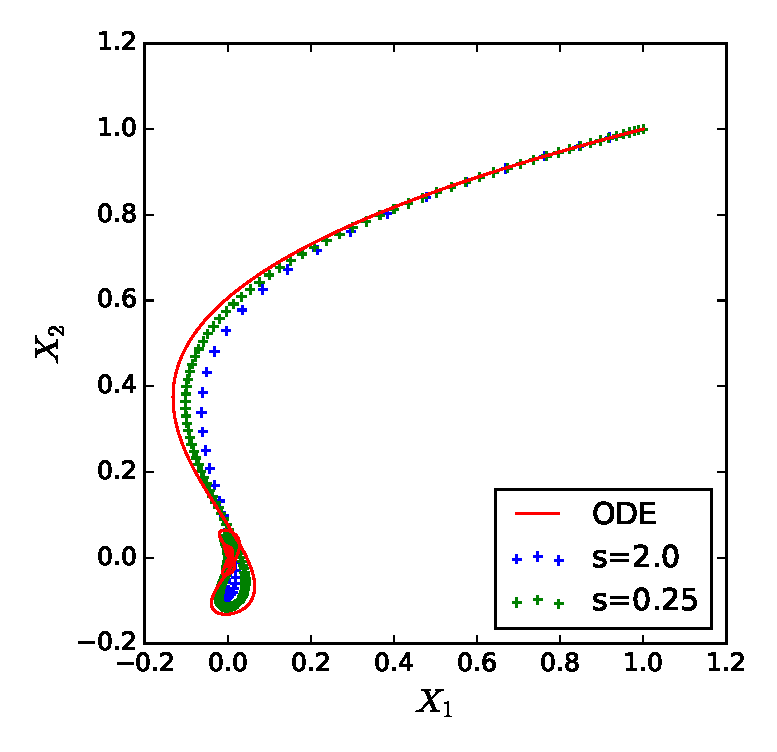
\includegraphics[width=0.6\linewidth]{Experiments/quadratic_traj_compare_annealed.eps}
\caption{}
\end{figure}
\end{frame}

\begin{frame}
\frametitle{An ODE for Nesterov Acceleration (II) [Us!]}
\begin{block}{Limit of ``Accelerated" Gradient Descent (for Strongly Convex $f$ )}
\begin{center}
$x_k \approx X(\overbrace{k\sqrt{s}}^{t})$ for the curve $X(t)$: \\
\begin{align*}
\begin{rcases*}
    x_k &= y_{k-1} - \overbrace{\frac{1}{\beta}}^{s} \nabla f(y_{k-1})\\
    y_k &= x_k + \frac{\sqrt{\kappa(\beta)}-1}{\sqrt{\kappa(\beta)}+1} (x_k - x_{k-1}) 
\end{rcases*} \overset{s \to 0}{\longrightarrow} \underbrace{\ddot{X}}_{``mass"} + \underbrace{2 \sqrt{\alpha} \dot{X}}_{``damping"} + \underbrace{\nabla f(X)}_{``force"} = 0
\end{align*}
\end{center}
\end{block}


\begin{block}{Lyapunov Functional (Strongly Convex) [Us!]}
\small{
$e^{\textcolor{red}{\sqrt{\alpha}} t} (f(X(t)) - f(x^*)) + \frac{\alpha}{2} ||X+\frac{1}{\sqrt{\alpha}} \dot{X} - x^*||_2^2 \implies f(X(t)) - f(x^*) \lesssim \mathcal{O}(e^{-\textcolor{red}{\sqrt{\alpha}} t})$}
\end{block}

\end{frame}

\begin{frame}
\frametitle{An ODE for Nesterov Acceleration (II) [Us!]}

\begin{block}{$f(X) = \frac{\alpha}{2} X^2 \equiv$ Damped Harmonic Oscillator!}
\begin{center}
\vspace{-.25cm}
\begin{align*}
   \ddot{X} + 2 \zeta \sqrt{\alpha} \dot{X} + \alpha X = 0 \implies 
\end{align*}
\vspace{-1cm}
\only<1>{
\begin{align*}
   X(t) = \begin{cases}
   & e^{-\zeta \sqrt{\alpha} t} \left( C \cos(\alpha(1-\zeta^2) t+\phi \right) \text{ when } \zeta < 1 \\
   & e^{-\zeta \sqrt{\alpha} t}(A+B t) \text{ when } \zeta = 1 \ \textcolor{red}{ \text{Nesterov Coefficient}} \\
   & A e^{ -(\sqrt{\alpha}(\zeta - \sqrt{\zeta^2-1})) t}+ B e^{ -(\sqrt{\alpha}(\zeta + \sqrt{\zeta^2-1}) t})   \text{ when } \zeta > 1
   \end{cases}
\end{align*}}

\only<2>{
\begin{align*}
   X(t) \sim \begin{cases}
   & e^{-\sqrt{\alpha} \zeta t}  \text{ when } \zeta < 1 \\
   & e^{-\sqrt{\alpha} t + \log t} \text{ when } \zeta = 1 \ \textcolor{red}{ \text{Nesterov Coefficient}} \\
   & e^{-\sqrt{\alpha}(\zeta - \sqrt{\zeta^2-1}) t}   \text{ when } \zeta > 1
   \end{cases}
\end{align*}}

\end{center}
\end{block}

\begin{block}{Nesterov ``Momentum" Coefficient \textit{is} Critical Damping (for $f(X) = \frac{\alpha}{2} X^2)  }
\begin{itemize}
\item $\zeta > 1$ Over-Damping -- Too Slow. 
\item $\zeta = 1$ Critical-Damping -- \textcolor{red}{Just Right}.
\item $\zeta < 1$ Under-Damping -- Too Much Oscillation.
\end{itemize}
\end{block}
\end{frame}

\begin{frame}
\frametitle{An ODE for Nesterov Acceleration (II) [Us!]}

\begin{block}{Nesterov ``Momentum" Coefficient \textit{is} Critical Damping }
\begin{figure}
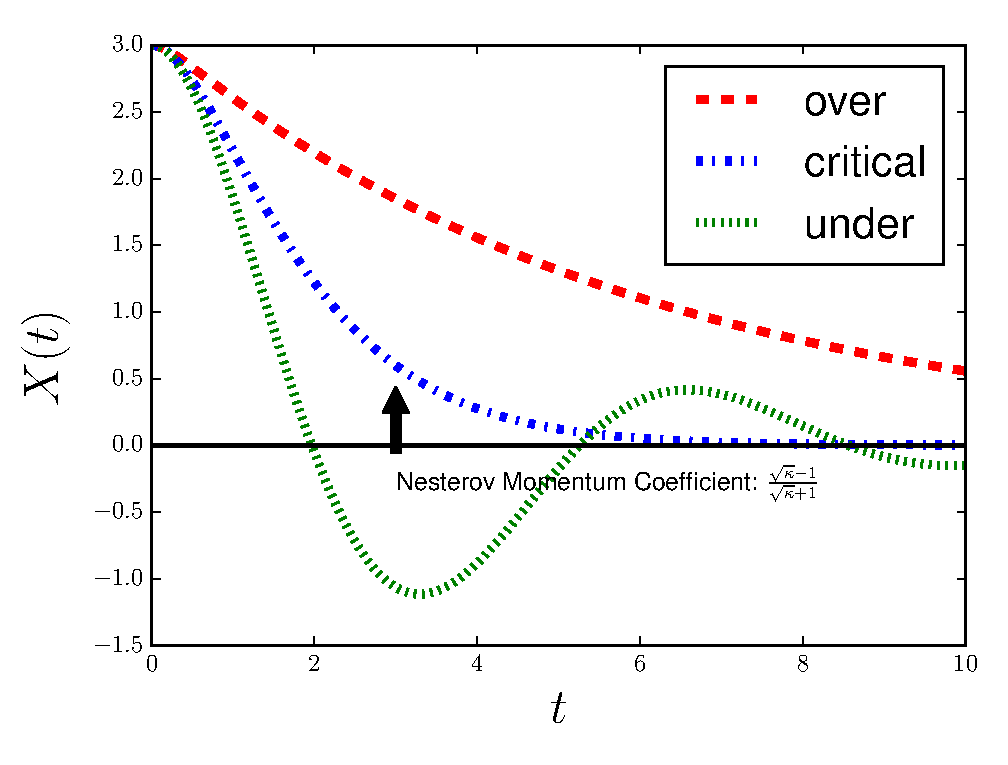
\includegraphics[width=0.8\linewidth]{Experiments/critical_damp_Nesterov.eps}
\caption{}
\end{figure}

\end{block}

\end{frame}

\section{Mirror Descent}

\subsection{Accelerated Mirror Descent}

\begin{frame}
\frametitle{Mirror Descent}
We want to extend these dimension-free convex optimization results to non-Euclidean spaces.
\begin{block}{Projected Gradient Descent}
For the Euclidean projection,
\begin{align*}
x_{k+1} &= \arg\min_{x \in C}\|x_k - s_k \nabla f(x_k) - x\|_2^2 \\
&= \arg\min_{x \in C} \langle x, \nabla f(x_k) \rangle + \frac{1}{s_k}\frac{\|x - x_k\|_2^2}{2}
\end{align*}
\end{block}
Our Euclidean norm in this case is acting as a distance function for projection.
\begin{block}{Bregman Divergence}
$$D_\Phi(x,y) = \Phi(x) - \Phi(y) - \nabla \Phi(y)^T(x-y)$$
\end{block}
\end{frame}

\begin{frame}
\frametitle{Mirror Descent Algorithm}
\begin{figure}
    \centering
    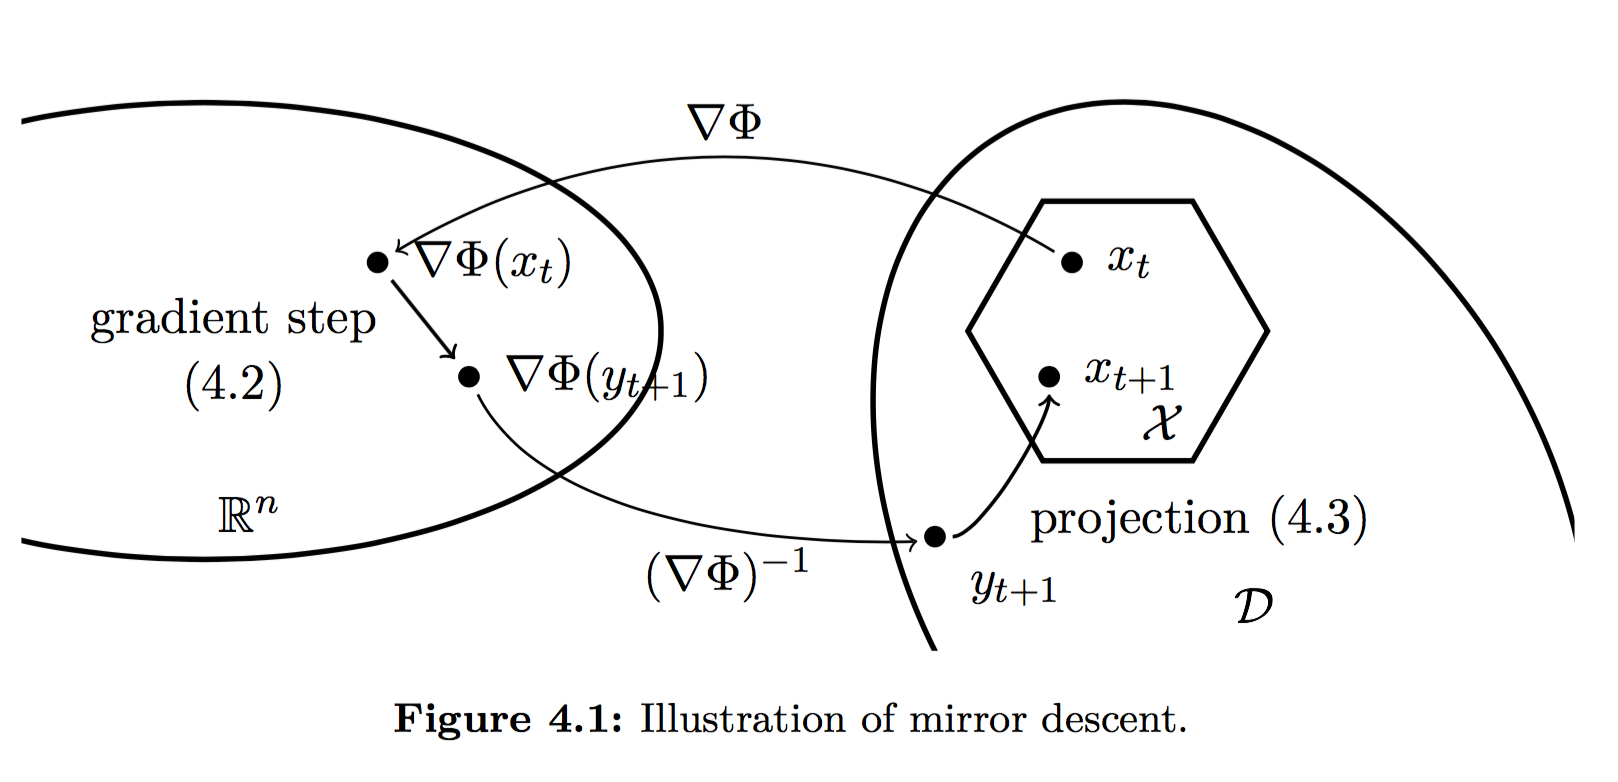
\includegraphics[width=0.9\textwidth]{Images/mda.png}
\end{figure}
\begin{block}{Mirror Descent Update}
$$x_{k+1} = \arg\min_{x \in D} \langle \nabla f(x_k), x \rangle + \frac{1}{s_k}D_{\Phi}(x,x_k)$$
\end{block}
\end{frame}

% - Formulate the Lyapanov function
% - A natural non-Euclidean generalization(ball setup, simplex) of the squared Euclidean norm is the Bregman Divergence(KL divergence is an example)

% - Mirror Descent:
\subsection{Mirror Descent ODE}
\begin{frame}
\frametitle{ODE for Accelerated Mirror Descent \cite{krichene2015accelerated}}
We generalize, using the Lyapunov function as our starting point
\[V(X(t),t) = t^2 (f(X(t)) - f^*) +  2 \|X(t)+\frac{t}{2}\dot X(t) - x^* \|^2\]
\begin{block}{Generalized Lyapunov \cite{krichene2015accelerated}}
\[V(X(t),Z(t),t) =t^2(f(X(t)) - f^*) + 4 D_{\psi^*} (Z(t), z^*) \]
\end{block}
\only<1> {Ensuring the properties of a Lyapunov function
\[\frac{d}{dt}V = 2 t (f(X) - f^*) + \textcolor{purple}{t^2} \langle \textcolor{red}{\nabla f(X)}, \textcolor{blue}{\dot X}\rangle + 4\langle\textcolor{red}{ \dot Z }, \textcolor{blue}{\nabla \psi^*(Z) - \nabla\psi^*(z^*)\rangle }\]
chose dynamics on dual variable \textcolor{red}{$\dot Z = -\frac{t}{2} \nabla f(X)$} and \textcolor{blue}{$\nabla \psi^*(Z) = X + \frac{t}{2} \dot X$} 
\[\frac{d}{dt}V \leq 0\]}
\only<2> {\begin{block}{Accelerated Mirror Descent ODE System \cite{krichene2015accelerated}}\begin{align*}
&\dot X = \frac{2}{t} (\nabla \psi^*(Z) - X)\\
&\dot Z = -\frac{t}{2} \nabla f(X)\\
&X(0) = x_0,~ Z(0) = z_0,~\nabla\psi^*(z_0) = x_0
\end{align*}
\end{block}}
\end{frame}

\begin{frame}
\frametitle{Accelerated Mirror Descent Discretization  \cite{krichene2015accelerated}}
A mixed forward/backward Euler scheme where $t_k = k\sqrt{s}$ and $\dot X(t_k) = \frac{X(t_k + \sqrt{s}) - X(t_k)}{\sqrt{s}}$
\begin{block}{Naive discretization via Euler method}
\only<1> {\begin{align*} x_{k+1}  &= \lambda_k \nabla \psi^*(z_k) + (1-\lambda_k) x_{k},\quad \lambda_k =\frac{2}{2+k}\\
z_{k+1}& = z_k -\frac{ks}{2} \nabla f(x_{k+1}) 
\end{align*}}
\only<2> {\begin{align*} x_{k+1}  &= \lambda_k \tilde z_k + (1-\lambda_k) x_{k},\quad \lambda_k =\frac{2}{2+k}\\
\tilde z_{k+1} &= \text{arg}\min_{x\in\mathcal{X}} \frac{ks}{2} \langle \nabla f(x_{k+1}), x \rangle + D_\psi (x, \tilde z_k)\\
\end{align*}}
\end{block}
Modified energy function $E_k = V(x_k,z_k,k\sqrt{s})$
\[E_{k+1} - E_k \leq 0 +\textcolor{red}{ D_{\psi^*}(z_{k+1},z_k)}\]
not readily shown to be a Lyapunov function
\end{frame}

\begin{frame}
\frametitle{Accelerated Mirror Descent Algorithm  \cite{krichene2015accelerated}}
\begin{block}{Accelerated Mirror Descent Algorithm \cite{krichene2015accelerated}}
\begin{align*} 
x_{k+1}  &= \lambda_k \tilde z_k + (1-\lambda_k) \tilde x_{k},\quad \lambda_k =\frac{2}{2+k}\\
\tilde z_{k+1} &= \text{arg}\min_{x\in\mathcal{X}} \frac{ks}{2} \langle \nabla f(x_{k+1}), x \rangle + D_\psi (x, \tilde z_k)\\
\tilde x_{k+1}&=\text{arg}\min_{x\in\mathcal{X}}\gamma s \langle \nabla f(x_{k+1}), x \rangle + R (x, x_{k+1})\\
\end{align*}
\end{block}
Modified energy function $\tilde E_k = V(\tilde x_k,z_k,k\sqrt{s})$
\[\tilde E_{k+1} - \tilde E_k \leq 0\]
\end{frame}

\begin{frame}
\frametitle{Mirror Descent on Simplex Constrained Problems}

\begin{columns}
\begin{column}{0.2\textwidth}
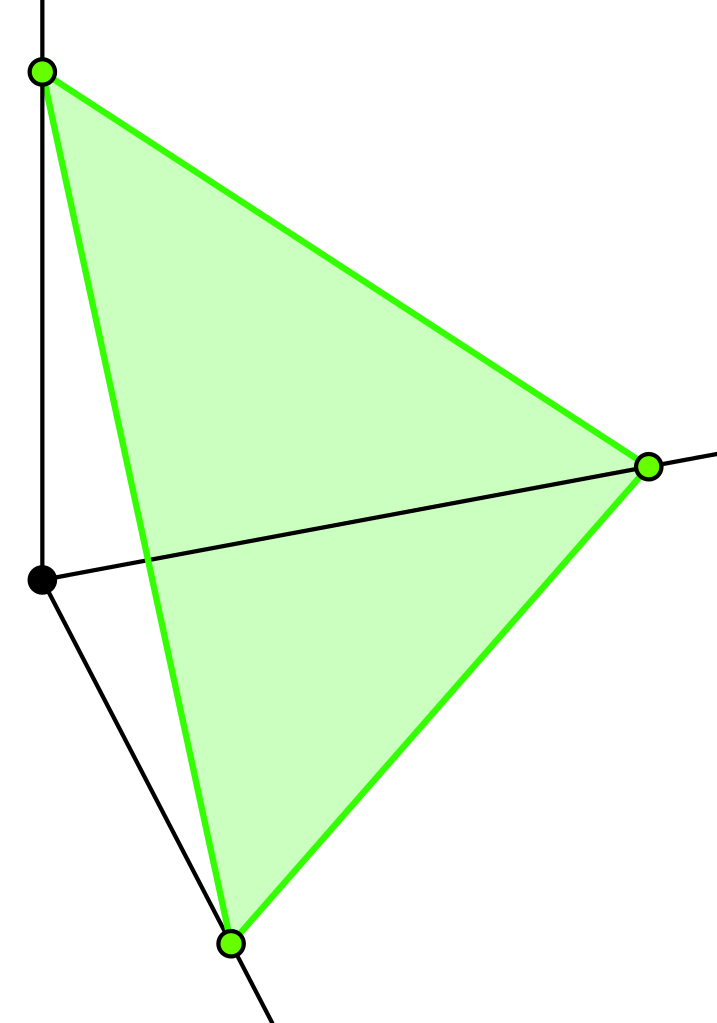
\includegraphics[width=0.8\linewidth]{Images/simplex.png}
\end{column}
\begin{column}{0.8\textwidth}  %%<--- here
    Simplex constrained problems are useful in tomography reconstruction, distributed routing, online learning, adversarial games
    
\end{column}
\end{columns}
%The mirror descent framework can be applied to simplex-constrained problems (tomography reconstruction, distributed routing, online learning, adversarial games). 
\begin{block}{Mirror Map: Negative Entropy on Simplex}
\begin{align*}
    &\Phi(x) = \sum_{i=1}^n x_i \log x_i + \delta (x|\Delta), \qquad \Phi^*(z) = \log \left(\sum_{i=1}^n e^{z_i} \right)\\
    &\nabla \Phi^*(z)_i = (\nabla \Phi)^{-1}_i = \frac{e^{z_i}}{\sum_{j=1}^ne^{z_j}}
\end{align*}
\end{block}
*smooth w.r.t. $\| . \|_\infty$
%Then $\psi^*$ is smooth w.r.t. $\| . \|_\infty$. For the regularization step, use $R(x,y) = D_\phi(x,y)$, with $\phi$ the smoothed negative entropy function
%\[\phi(x) = \epsilon \sum_{i=1}^n (x_i+\epsilon)\log(x_i+\epsilon)+\delta(x|\Delta)\]
\end{frame}

\begin{frame}
\frametitle{Numerical Experiments}
Mirror Descent for the simplex constrained log-sum-exp function with $x\in\mathbb{R}^3$, $I=100$ $f(x) = \log \left( \sum_{i=1}^I \langle a_i,x\rangle + b_i \right)$.
\begin{center}
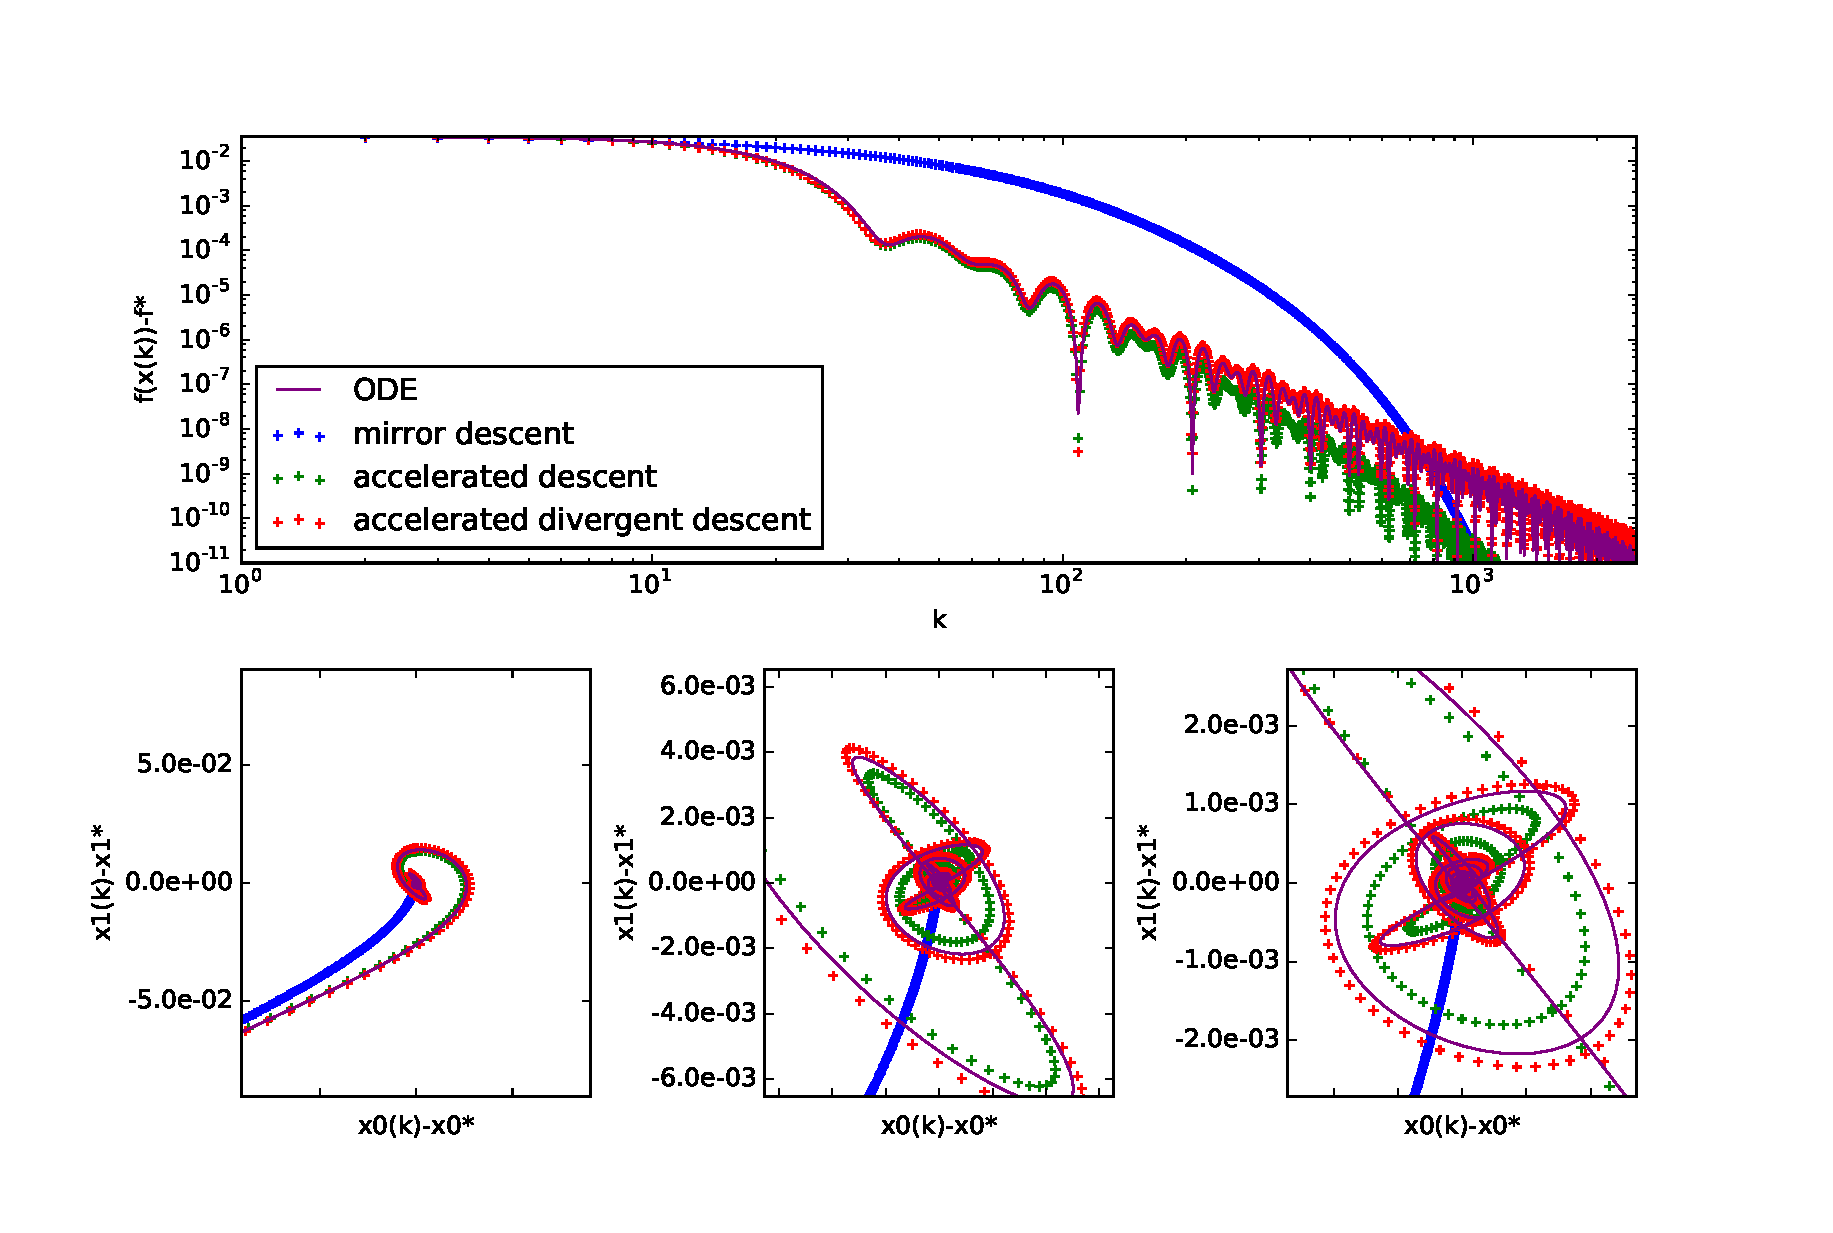
\includegraphics[width=0.87\linewidth]{Experiments/amd-all.eps}
\end{center}
\end{frame}

\begin{frame}
\frametitle{Conclusion}

\begin{block}{Key Takeaways}
\begin{enumerate}
    \item Reviewed accelerated first-order methods in discrete and continuous time
    \item Extended results in the Euclidean case to strongly convex functions
    \item Investigated mirror descent in the continuous and discrete time settings
\end{enumerate}
\end{block}

\huge{
How do we discretize from Continuous-Time ODE's $\to$ Useful Optimization Algorithms?
}

\end{frame}

\begin{frame}[t, allowframebreaks]
\frametitle{References}
\footnotesize{
\bibliographystyle{amsalpha}
\bibliography{refs.bib}
\cite{*}}
\end{frame}


\end{document}

